\documentclass[english,11pt,a4paper]{article}
\usepackage{preamble}

%-------------------------------------------------------------------------%
% MASTERARBEIT (╯°□°)╯︵ ┻━┻       ┬─┬ノ( º _ ºノ)      (ノಠ益ಠ)ノ彡┻━┻   %
%-------------------------------------------------------------------------%

\begin{document} %------------   \(◕ ◡ ◕\)   -----------------------------%
% (/◔ ◡ ◔)/   ◕‿◕

Version 4 \scriptsize \hfill Juri; Hyperelliptic Curves --- Draft --- \today
\normalsize

\section{Addition Law}

\subsection{Definitions and Notation}

\begin{defin}
	Let $K$ be a field with char$(K) \neq 2, 3$ and $\bar K$ its algebraic closure. Define the hyperelliptic curve of genus two $\enk$ as the set of solutions in $K^2$ to the equation $y^2=C(x)$ where $C(x)=x^5+ax^4+bx^3+cx^2+dx+e$ is a polynomial over $K$. Similarly, the set of solutions in the closure would be denoted $\enkb$.	Define $\ek$ as $\enkb \cup \{ \infty \}$.

	To avoid a clash of notations, we call $\ii$ the infinity that we use in $K \cup \{ \ii \}.$

	\textbf{Note} that we could obtain a more reduced form of $C(x)$, eliminating $a$ by shifting $x$ to $x-a/5$. However, since this would rob us of the possibility of char$(K) = 5$ without simplifying our coming calculations in any significant manner, we shall be reluctant towards using this trick.

	For the purpose of clarity, let points on the hyperelliptic curve --- in the sense of solutions to $y^2=C(x)$ --- be designated by the calligraphic letter $\q=(x,y) \in \enkb$. The point opposite to $\q$ will be written $\bar \q = (x,-y)$ and by symmetry of the curve in $y$ also belongs to $\enkb$. In the case where $\q = \infty$, define $\bar \q = \infty$.

	We want to consider the set of all pairs $(\q_1,\q_2)$ and tame it with an equivalence relation with the goal of obtaining an additive group:
\end{defin}
% \vspace{2mm}
\begin{defin}\label{defj}
	Define $\J$ to be the set\scalebox{1.3}{ $\nicefrac{ \j }{\sim }$ }where $\j = \ekb \times \ekb$. It is called the ``Jacobian'' and the equivalence relation is defined by
	\begin{align*}
		(\q_1,\q_2) &\sim (\q_2,\q_1) \\
		\text{and\hspace{5mm}} (\q,\bar \q) & \sim ( \infty , \infty ). 
	\end{align*}
	Write $\{ \q_1,\q_2 \}$ from now on and let bold letters denote points on the curve in the sense of classes of unordered pairs $\P =\{ \q_1, \q_2 \} \in \J$. The point $\{ \bar \q_1, \bar \q_2 \}$ will be called $\bar \P$ for now but can already tentatively be thought of as $-\P$. Call $\{ \infty, \infty \}$ the zero of our set. Call $\q_i$ a point-component.% We will also permit ourselves the notation $\{ \q,\bar \q \} = 0$ and we refrain from explicitly stating that $\P$ is in fact an equivalence class.

	A point $\q = (x_0,y_0)$ is called singular if it fulfills both $y_0=0$ and $C'(x_0) = 0$. A curve is called singular if and only if it has a singular point. We consider only non-singular hyperelliptics from here on; this amounts to $C(x)$ having no repeated factors over $\bar K$ (``squarefree)''.%xxx
\end{defin}

\subsection{The General Case}

Let's start with $\P_1 = \{\q_1,\q_2\}$, $\P_2 = \{\q_3,\q_4\}$ with $\q_i = (x_i,y_i) \in \enk$ or $\q_i = \infty$. To define $\P_3 = \P_1 + \P_2$ we distinguish between one general case and a number of special cases and first derive the results of the former before enumerating the latter ones.

\begin{case} {\scshape Four Distinct Point-Components:}
	Let $\q_i \in \enk$ and $\P_i$ be defined as above with $x_i \neq x_j$ whenever $i \neq j$.

	The overarching idea is to obtain a fifth and sixth $x$-coordinate and the corresponding $y$-coordinates by passing a polynomial of degree three through the four points $\q_i$. Ideally this should give us two additional intersections with the curve which we then use as the components of our point $\P_1 + \P_2$.

	{\scshape Step 1:} It is known that the Vandermonde matrix
	\begin{align*}V=
		\begin{pmatrix}
			1 & x_1 & x_1^2 & x_1^3\\
			1 & x_2 & x_2^2 & x_2^3\\
			1 & x_3 & x_3^2 & x_3^3\\
			1 & x_4 & x_4^2 & x_4^3\\
		\end{pmatrix}
	\end{align*}
	has determinant $\prod_{i < j} (x_i-x_j)$ which is conveniently non-zero if and only if the $x_i$ are pairwise distinct. Let $p(x) = p_3 x^3 + p_2 x^2 + p_1 x + p_0 \in \bar K[x]$ be the polynomial in unknown coefficients that we are looking for. With $\textbf{y} = (y_1 \ y_2 \ y_3 \ y_4)^t$ and $\textbf{p} = (p_0 \ p_1 \ p_2 \ p_3)^t$, the problem of determining $p(x)$ can be rewritten as
	\begin{align*}
		V \cdot \mathbf{p} = \mathbf{y}
	\end{align*}
	which by invertibility of $V$ has a unique solution for $\mathbf{p}$ with $p_i\in K$.

	\textbf{Note} that the leading coefficient of $p(x)$ is
	\begin{align*}
	  p_3 = \frac{1}{\det (V)}
	  \begin{vmatrix}
			1 & x_1 & x_1^2 & y_1\\
			1 & x_2 & x_2^2 & y_2\\
			1 & x_3 & x_3^2 & y_3\\
			1 & x_4 & x_4^2 & y_4\\	  
	  \end{vmatrix}
	\end{align*}
	and the next step will depend on whether $p(x)$ is truly of degree 3 or not.

	{\scshape Step 2a:} Knowing the coefficients $p_i$ of $p(x)$ we first assume that $p_3 \neq 0$, so can proceed to look for the two additional solutions of the sextic equation
	\begin{align*}
		\tag{$\ast$} \label{sex} C(x)-\left ( p(x) \right )^2 = 0.
	\end{align*}
	Observe that this vanishes at $x_1, x_2, x_3$ and $x_4$, so write the lefthand side as
	\begin{align*}
		C(x)-\left(p(x)\right)^2 = -p_3^2(x-x_1)(x-x_2)(x-x_3)(x-x_4)(x-x_5)(x-x_6)
	\end{align*}
	 for $x_5$ and $x_6$ in $\bar K$. Comparing the coefficients of both expressions at $x^4$ and $x^5$ yields
	\begin{align*}
		\label{four} \tag{4} \sum_{\substack{i,j=1\\i<j}}^6 x_i x_j &= T_4\\
		\tag{5} \text{and\hspace{5mm}} \sum_{i=1}^6 x_i &= T_5\\
	\end{align*}
	where $T_4 = \frac{p_2^2+2 p_1 p_3-a}{p_3^2}$ and $T_5 = \frac{1-2 p_2 p_3}{p_3^2}$.
	The first expression gives
	\begin{align*}
		x_6 \sum_{i=1}^5 x_i + \sum_{\substack{i,j=1\\i<j}}^5 x_i x_j = T_4.
	\end{align*}
	Doing this twice and replacing $x_6$ with the information from (5) gives the tidy quadratic equation

	\vspace{-3mm}
	\fline
	\begin{align*}
		\tag{$\dag$} \label{dagger} x^2 - \left(T_5 - \sumfo \right) \cdot x+ \left(T_4 - T_5 \sumfo + \sum_{\substack{i,j=1\\i\leq j}}^4 x_i x_j \right) = 0
	\end{align*}
	\fline

	of which $x_5$ is one solution and --- by symmetry of the above steps --- $x_6$ the other one. Compute $y_i=p(x_i)$, $i=5,6$ to obtain $\q_5 = \{ x_5, -y_5 \}$ and $\q_6 = \{ x_6, -y_6 \}$, at which point it becomes clear that the worst-case scenario for our field extension to accommodate the new coordinates is to be quadratic. Finally we define $\P_1 + \P_2$ to be equal to $\P_3 = \{ \q_5, \q_6 \}$.

	{\scshape Step 2b:} If $p_3$ were zero, the equation \eqref{sex} would be quintic instead. We may therefore write the lefthand side as $(x-x_1)(x-x_2)(x-x_3)(x-x_4)(x-x_5)$, again for $x_5$ somewhere in $\bar K$. Defining $T_{4\infty}=p_2^2 - a$ and comparing the coefficients at $x^4$ gives

	\vspace{-3mm}
	\fline
	\begin{align*}
		\tag{$\ddag$} \label{dagger2} x_5 = T_{4\infty} - \sum_{i=1}^4 x_i
	\end{align*}
	\fline

	and we may rejoice in the implication of $x_5$ staying in $K$.

	Compute $y_5 = p(x_5)$ and define $\P_1 + \P_2$ to be the point $\P_3 = \{ (x_5, y_5), \infty \}$.

	{\scshape Step $1'$:} To extend our construction from $\enk$ to $\ek$ we now consider $\q_4 = \infty$ with the other $\q_i = (x_i,y_i)$ as before. This can be seen as the $x_i$ still being pairwise distinct, only that one of them is allowed to be $\ii$ here.

	There is no coordinate $x_4$ this time, so we pass a quadratic polynomial $p(x)$ through the remaining three points $(x_i,y_i)$. This means that we solve the linear system $\tilde V \cdot \mathbf{p} = \tilde \mathbf{y}$ where $\tilde V$ is the Vandermonde matrix for $x_i$, $i=1,..,3$ which incidentally is the upper-left 3$\times$3 sub-matrix of $V$. Here $\mathbf{p}=(p_0 \ p_1 \ p_2)^t$ and $\tilde \mathbf{y}=(y_1 \ y_2 \ y_3)^t$ are defined as expected.

	As before, the leading coefficient of $p(x)$ might or might not be zero, 
	%but this time, dear reader, let us not give a toss
	but \eqref{sex} will be quintic in either case, so we only have to worry about one step 2.

	{\scshape Step $2'$:} Doing a coefficient comparison at $x^3$ and at $x^4$ in \eqref{sex} gives
	\begin{align*}
	  \tag{$3'$} \sum_{\substack{i,j=1\\i<j}}^3 x_i x_j + x_5\sum_{i=1}^3 x_i + x_5 x_6 &= b-2p_1 p_2\\
	  \tag{$4'$} \text{ and\hspace{5mm}}
	  \sum_{i=1}^3 x_i + x_5 + x_6 &= p_2^2-a.
	\end{align*}
	Call the righthand terms $T_{3\infty}$ and $T_{4\infty}$, combine both equations and obtain

	\vspace{-2mm}
	\fline
	\begin{align*}
		\label{daggerp} \tag{$\dagger '$} x^2 - \left( T_{4\infty} \sumthr \right) \cdot x + \left(T_{3\infty} - T_{4\infty} \sumthr + \sum_{\substack{i,j=1\\i\leq j}}^3 x_i x_j \right)
	\end{align*}
	\fline

	Solve, call the two solutions $x_5$ and $x_6$, compute $y_5$ and $y_6$ through $p(x_5)$ and $p(x_6)$ and define $\P_1+\P_2$ to be $\P_3=\{ (x_5,-y_5) , (x_6,-y_6) \}=\{ \q_5, \q_6 \}$.
\end{case}

\begin{center}
$\sim$
\end{center}


\begin{figure}[ht!]
	\fline
	\begin{center}
		\vspace{1mm}
		% \framebox{The eight cases illustrated}
		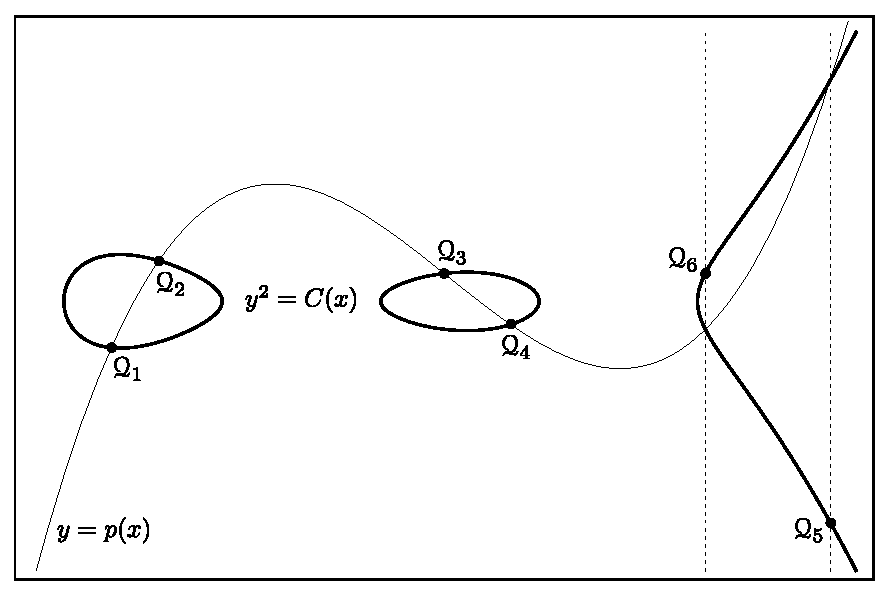
\includegraphics[width=0.9\textwidth]{addition_general.pdf}

		{\scshape Figure 1a}: The general case for the addition law in $\mathds{R}^2$ where $p_3 \neq 0$.

		\vspace{1mm}

		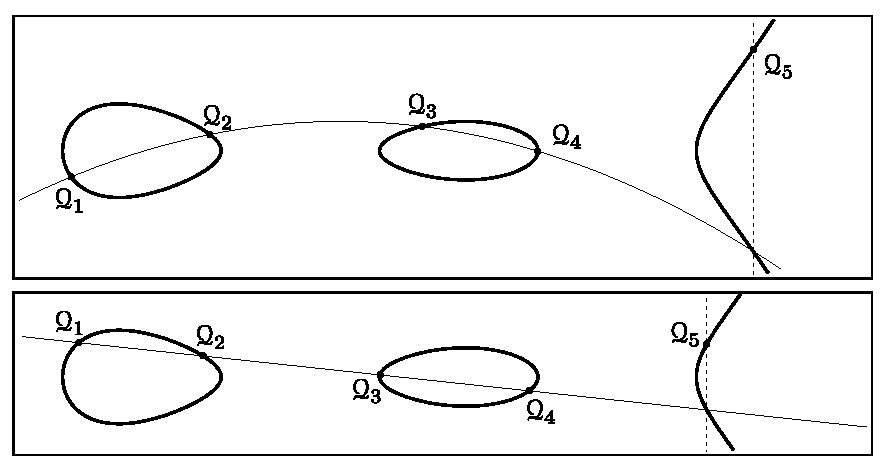
\includegraphics[width=0.9\textwidth]{addition_quadr_and_lin.pdf}

		{\scshape Figures 1b} and {\scshape 1c}: If $p_3 = 0$ we have at most five intersections.
	\end{center}
	\vspace{-1.5mm}
	\fline
\end{figure}


\begin{remark}
	Up to this point, we have only given the general-case rule for elements in $\ek \times \ek$. Extending to $\j = \ekb \times \ekb$ is trivial as we can simply choose $\bar K$ as the new $K$. The final step is to note that everything until now is well-defined on $\J$. The equivalence relation from Definition \ref{defj} corresponds to interchanging $\q_1$ and $\q_2$ or $\q_3$ and $\q_4$ or both.
	To this end we can check that interchanging $(x_i,y_i) \rightleftharpoons (x_j,y_j)$ does nothing to the resulting $\q_5$ and $\q_6$. This is the case because $p(x)$ does only depend on the solution of the linear system $V \cdot \mathbf{p} = \mathbf{y}$ on which the aforementioned permutation has no effect. With $p$ invariant, the subsequent steps remain unchanged as well.

	Finally, the restriction to $K$ instead of $\bar K$ was to showcase the degree of the required field extension, a feat we will now leave aside by always using $\bar K$.
\end{remark}


	%\textbf{Note} also that solving either of the dagger equations does not guarantee that the resulting $x_5$ or $x_6$ differ from the other $x_i$ or even from each other. In fact the situation may very well arise where for instance $x_6 = x_1$ because $p(x)$ happens to be tangential to the curve at $x_1$. The equation \eqref{sex} would then factor as $-p_3^2(x-x_1)^2\prod_{i=1}^5 (x-x_i)$.

% \newpage
Before we begin listing the special cases, we impose the following property: The sum of any $\P_1 = \{\q_1,\q_2\}$ and $\P_2 = \{\q_3,\q_4\}$ in $\J$ fulfills the equality
\begin{align*}
	\tag{$\diamondsuit$} \label{switch} \P_1 + \P_2 &= \{\q_3,\q_2\} + \{\q_1,\q_4\}.
\end{align*}
Note that the general-case addition we just defined already fulfills this, as we noted before that interchanging any of the $(x_i, y_i)$ does not impact the solution $\mathbf{p}$ of the linear system nor any of the dagger equations.

\begin{remark}\label{permut}
	The property \eqref{switch} corresponds to the permutation $(1 \, 3)$ on the point-components $\q_i$. With Definition \ref{defj} allowing the permutations $(1 \, 2)$ and $(3 \, 4)$ this naturally leads to the observation that in fact all permutations of point-components must now leave the sum unchanged. It is easy to check that the three transpositions generate all of $S_4$ and the previous remark already provides compatibility with the construction of the general case.

	A substantial bonus of this is the fact that commutativity corresponds to the permutation $(1 \, 3)(2 \, 4)$ which by the above we now obtained for free.
\end{remark}

%xxx not 100\% satisfactory...I really want to show that this is not only justified but  inevitable.

% \newpage

\subsection{Complete List of Cases}

We may now impose conditions on the relations between the $\q_i$ without mentioning whether they belong to $\P_1$ or $\P_2$. As a result, the list of special cases can be written in a significantly more concise manner.

As we strive to define $\{ \q_1 , \q_2 \} + \{ \q_3 , \q_4 \}$, for any $\q_i = (x_i,y_i) \in \enkb$ or $\q_i = \infty \in \ekb$ we observe that the following simplification takes place:

Let $\{ i,j,k,l \}=\{ 1,2,3,4 \}$. Whenever $\q_i = \bar \q_j$ for $i \neq j$ we define
\begin{align*}
  \{ \q_1 , \q_2 \} + \{ \q_3 , \q_4 \} &= \{ \q_k , \q_l \} + \{ \q_i , \bar \q_i \}\\
  &= \{ \q_k , \q_l \} + \{ \infty, \infty \}.
\end{align*}
The justification for this follows directly from Remark \ref{permut} and Definition \ref{defj}. It is easily checked that this sum remains well defined if the choice of $i$ and $j$ is not unique. This allows us to treat the above as a separate case in order to characterize the other cases solely through the $x$-coordinates of the $\q_i$, so
\begin{align*}
  x_i = x_j \iff \q_i = \q_j
\end{align*}
for any $\q_i, \q_j \in \ekb$ provided we assign $\q_i = \infty$ the $x$-coordinate $x_i = \ii$.

We may now write the distinction between the remaining cases as follows:

\begin{enumerate}
	\parskip 1mm
	\item The general case where all $x_1,..,x_4$ are pairwise distinct.
	\item The case $x_i = x_j$ but $x_i$, $x_k$ and $x_l$ are pairwise distinct.
	\item The case where $x_i = x_j$ and $x_k = x_l$ but $x_i \neq x_k$.
	\item The case $x_i = x_j = x_k$ but $x_l \neq x_i$.
	\item The case where $x_1 = x_2 = x_3 = x_4$.
\end{enumerate}
\parskip 3mm

Since we are allowed to permute point-components anyway, we may fix which of the $\q_i$ are equal and write everything out for the complete and final list:

\vspace{-3mm}
\fline
% \vspace{-2mm}
\begin{enumerate}\setcounter{enumi}{-1}
	\parskip 1mm
	\item The addition with zero, i.e. $\{ \q_1, \q_2 \} + \{ \infty, \infty \}$, $\q_1$, $\q_2 \in \ekb$.
	\item The general case where $\q_i \neq \q_j$ and $\q_i \neq \bar \q_j$ for $i \neq j$.
	\item The single tangential case where all $\q_i$ as in case 1 with the exception of $\q_1 = \q_2 \in \enkb$ with $y_1 \neq 0$.%the remaining $\q_3$, $\q_4 \in \ek$ are both distinct from each other as well as from $\pm \q_1, \bar \q_3$ and $\bar \q_4$.
	\item The double tangential case where all $\q_i$ as in case 1 with the exception of $\q_1 = \q_2 \in \enkb$ with $y_1 \neq 0$ and $\q_3 = \q_4 \in \enkb$ with $y_3 \neq 0$.% and $\q_1 \neq \pm \q_3$.
	\item The triple point case wherein $\q_1=\q_2=\q_3 \in \enkb$ with $y_1 \neq 0$ and $\q_4 \in \ekb$ differs from both $\q_1$ and $\bar \q_1$.
	\item The quadruple case where all $\q_i \in \enkb$ are equal with $y_i\neq 0$.
\end{enumerate}
\vspace{-2mm}
\fline
\parskip 3mm

\begin{remark}\label{rem}\hfill
\begin{enumerate}[(i)]
	\item In both lists, the cases do not overlap.
	
	\item For the list to be complete, we must allow for $\q_i = \infty$ for some $i$. Note that one is sufficient, since if two or more $\q_i$ were to be $\infty$, we would be back at the case 0 by virtue of \eqref{switch}, bringing the two infinities together in one point. As for case 1, we consider $\q_i \in \enkb$ and $\q_i \in \ekb$ in two separate cases and postpone handling the latter.\label{extend}

	\item As for the first case, the constructions will a priori only be made on $\j$. It remains to check that this makes indeed for a well-defined addition on $\J$ by being invariant under the permutations $\q_i \rightleftharpoons \q_j$ for any $i$, $j$.
\end{enumerate}
\end{remark}

\subsection{Addition Law for the Special Cases}

Before we handle the next construction steps we need an intermediate result.
\vspace{-8mm}
\begin{lemma}\label{div}
  If $D(\tau) = D'(\tau) = \dots = D^{(k-1)}(\tau) = 0$ for a polynomial over a field of characteristic $0$ or $p \geq k$ then
  \begin{align*}
    (t - \tau)^k \mid D(t).
  \end{align*}
  \begin{proof}
    Assume $\tau = 0$ by shifting $t$ to $t + \tau$. Now $D(t) = \sum_{i=0}^d a_i t^i$. Now
    \begin{flalign*}
      &&a_i = \frac{1}{i!} D^{(i)}(0) = 0 \text{\hspace{25mm}} i = 0 ,.., k-1
    \end{flalign*}
    so $t^k$ divides $D(t).$
  \end{proof}
\end{lemma}

We will now use this property for $D(x)= C(x) - p^2(x)$ when factoring \eqref{sex}.

\setcounter{case}{-1}

\begin{case}
  {\scshape Addition with Zero:} As one might have anticipated we define $\P_1 + \P_2 = \P_1$ for every $\P_1 \in \J$ if $\P_2 = \{\infty, \infty\} = 0$.
\end{case}

\setcounter{case}{1}
\begin{case}
	{\scshape Tangential:} Let $\q_i\in \enkb, \q_1 = \q_2$, $y_1 \neq 0$ but $x_1$, $x_3$ and $x_4$ are pairwise distinct. We cannot use the Vandermonde matrix in this case because it won't possess maximal rank, consequently being non-invertible. We can however obtain an additional equation by demanding that our polynomial $p(x)$ be tangential to the curve at $\q_1$. This gives
	\begin{align*}
	  2 y \frac{dy}{dx} &= 5  x^4 + 4 a x^3 + 3 b x^2 + 2 c x + d \\
	  \text{and\hspace{8mm}} \frac{dy}{dx} &= 3 p_3 x^2 + 2 p_2 x + p_1
	\end{align*}
	meaning that the system to solve for $\mathbf{p}$ is now $\Vdoub \cdot \mathbf{p} = \ydoub$ with
	\begin{align*}\Vdoub=
		\begin{pmatrix}
			1 & x_1 & x_1^2 & x_1^3\\
			0 & 1 & 2 x_1 & 3 x_1^2\\
			1 & x_3 & x_3^2 & x_3^3\\
			1 & x_4 & x_4^2 & x_4^3\\
		\end{pmatrix}.
	\end{align*}
	The subscript indicates at which points the intersections have higher order.
	Here $\ydoub$ is defined as $\mathbf{y}$ with $y_2$ replaced by $y_2'=\frac{C'(x_1)}{2 y_1}$ where $C'(x)$ is the derivative of $C$ and $2y_1 \neq 0$ because char$(\bar K) \neq 2$ and $y_1\neq 0$. Since $\det(\Vdoub) = (x_4-x_1)^2(x_3-x_1)^2(x_4-x_3)$ this fits neatly into our constraints by being non-zero exactly in the case where $x_1, x_3$ and $x_4$ are pairwise distinct.

	Once the polynomial is determined, we note that the $p^2(x)$ shares a tangent with $C(x)$ at $x_1$ on purpose, specifically
	\begin{align*}
	  D'(x_1) &= C'(x_1) - 2 p(x_1)p'(x_1)\\
	  				&= C'(x_1) - 2 y_1 y_2' = 0
	\end{align*}
	so we use Lemma \ref{div} to see that the lefthand side of \eqref{sex} either factors as $-p_3^2(x-x_1)^2\prod_{i=3}^6(x-x_i)$ or $(x-x_1)^2\prod_{i=3}^5(x-x_i)$. Now step two will be entirely identical to that of the general case and we can again solve \eqref{dagger2} or \eqref{dagger} for $x_5$ or $x_5$ and $x_6$.
\end{case}

\begin{case}
	{\scshape Double Tangential:} Let $\q_i \in \enkb$, $\q_1 = \q_2$ and $\q_3 = \q_4$ but $x_1 \neq x_3$ and $\q_i \neq \bar \q_i$ meaning that neither $y_1$ nor $y_3$ will be zero. As before, we lack equations for our linear system, requiring the use of a second tangential constraint. Replace the fourth row of $\Vdoub$ and $\ydoub$ exactly like we did for the second one: $y_4'=\frac{C'(x_3)}{2 y_3}$ and
	\begin{align*}\Vddoub=
		\begin{pmatrix}
			1 & x_1 & x_1^2 & x_1^3\\
			0 & 1 & 2 x_1 & 3 x_1^2\\
			1 & x_3 & x_3^2 & x_3^3\\
			0 & 1 & 2 x_3 & 3 x_3^2\\
		\end{pmatrix}.
	\end{align*}

	Now $\det(\Vddoub)=(x_3-x_1)^4$ and this is again different from zero precisely whenever $x_3 \neq x_1$, so as before solve $\Vddoub \cdot \mathbf{p} = \yddoub$ for $\mathbf{p}$, then note that $D(x)$ has double zeroes at $x_1$ and $x_3$ by the same argument as in case 2.
	% \begin{align*}
	%   D'(x_3) = C'(x_3) - 2 y_3 y_3' = 0
	% \end{align*}
	By Lemma \ref{div} we know that \eqref{sex} has a factor $(x-x_1)^2(x-x_3)^2$ so we use the same procedure of case 1 with $x_2 = x_1$ and $x_4 = x_3$ to solve \eqref{dagger} or \eqref{dagger2}.
\end{case}

\begin{case}
	{\scshape Triple Point:} Let $\q_i \in \enkb , \q_1=\q_2=\q_3$ but $x_1 \neq x_4$ and $y_1 \neq 0$. We can thus see this as a third-order intersection and demand that the curve and the polynomial share a second-order derivative at $\q_1$:
	\begin{align*}\Vtri=
			\begin{pmatrix}
			1 & x_1 & x_1^2 & x_1^3\\
			0 & 1 & 2 x_1 & 3 x_1^2\\
			0 & 0 & 2 & 6x_1\\
			1 & x_4 & x_4^2 & x_4^3\\
		\end{pmatrix}.
	\end{align*}
	Here $\det(\Vtri)=2(x_4-x_1)^3$ and with this, define $\ytri$ by taking $\ydoub$ and replacing the third coordinate by $y_3'' = \frac{C''(x_1)}{2y_1}-\frac{(C'(x_1))^2}{4y_1^3}$ where $C''(x)$ is the second-order derivative of $C$.

	Apply Lemma \ref{div} as in case 2, only this time we also have
	\begin{align*}
	  D''(x_1) &= C''(x_1) - 2 p(x_1)p''(x_1) - 2 (p'(x_1))^2\\
	  				 &= C''(x_1) - 2 y_1 y_3''- 2(y_2')^2 = 0
	\end{align*}
	as can be checked by glancing at the definition of $y_3''$. With \eqref{sex} factoring as $-p_3^2(x-x_1)^3\prod_{i=4}^6(x-x_i)=0$ or $(x-x_1)^3\prod_{i=4}^5(x-x_i)=0$, this again allows us to continue with one of the second steps of case 1 to find $\P_3$.
\end{case}

\begin{case}
	{\scshape Quadruple Point:} Given the situation where $\q_i = \q_1 \in \enkb$ for every $i$ with $y_1 \neq 0$, we use
	\begin{align*}\Vquad &=
		\begin{pmatrix}
			1 & x_1 & x_1^2 & x_1^3\\
			0 & 1 & 2 x_1 & 3 x_1^2\\
			0 & 0 & 2 & 6x_1\\
			0 & 0 & 0 & 6\\
		\end{pmatrix}
	\end{align*}
	which is invertible in all fields but those of characteristic 2 and 3.

	Here $\yquad$ is the same as $\ytri$ except for the last coordinate which should read
	\begin{align*}
		y_4''' = \frac{C'''(x_1)}{2y_1}-\frac{3C'(x_1)C''(x_1)}{4y_1^3}+\frac{3(C'(x_1))^3}{8y_1^5}
	\end{align*}
	where $C'''(x)$ is the third-order derivative of $C$. Once more, we solve the linear system $\Vquad \cdot \mathbf{p}=\yquad$. In addition to $D^{(i)}(x_1)=0$, $i=0,..,2$ we have
	\begin{align*}
	  D'''(x_1) = C'''(x_1) - 2 y_1 y_4''' - 6 y_2' y_3'' = 0
	\end{align*}
	so $D(x) = -p_3^2(x-x_1)^4(x-x_5)(x-x_6)$ or $D(x)=(x-x_1)^4(x-x_5)$ which we subsequently use to solve \eqref{dagger} or \eqref{dagger2} and we're done.
\end{case}
% \vspace{-4mm}
\begin{center}
$\sim$
\end{center}

  \textbf{Finally}, as noted in Remark \ref{rem}, \eqref{extend} we have yet to extend our definition from $\enkb$ to $\ekb$. Observe that this is only relevant for cases number two and four where we now consider $\q_4 = \infty$ as we did in {\scshape Step $1'$} of the general case. As an analogue to this, the relevant matrices $\tilde V_1$ and $\tilde V_{11}$ will be the upper-left $3 \times 3$ sub-matrices of their $\enkb$-counterparts $V_1$ and $V_{11}$.

  In both cases we obtain a linear system of the form $\tilde V_{\ast} \cdot \mathbf{p} = \tilde \mathbf{y}_{\ast}$ for a three-element vector $\mathbf{p}$ and the vectors $\tilde \mathbf{y}_{1}$ and $\tilde \mathbf{y}_{11}$ are defined like their 4-element counterparts $\mathbf{y}_{1}$ and $\mathbf{y}_{11}$ with the last coordinate omitted.

  Both matrices $\tilde V_{\ast}$ are invertible and we therefore get a unique polynomial $p(x)$ wich we use to solve \eqref{daggerp}, obtaining $x_5$, $x_6$, $y_5=p(x_5)$ and $y_6=p(x_6)$ in $\bar K$ and we define $\{ \q_1 , \q_2\}+\{ \q_3 , \infty \} = \{ \q_5 , \q_6 \} = \{(x_5,-y_5),(x_6,-y_6)\}$.

\subsection{Well-Definedness of the Addition Law}

To check whether our addition is well defined on $\J$ in each of the cases, we have to consider the permutation of point-components $\q_i$ under the equivalence relation from Definition \ref{defj}. Furthermore, to claim that all possible cases are all covered, it is necessary to check the permutations under \eqref{switch}. Both cases can be combined into a single one by the following statement:

\textbf{Lemma:} In each given definition of `$+$', the result is invariant under the permutation $\q_i \rightleftharpoons \q_j$.

\begin{proof}
  Simultaneously interchanging $x_i \rightleftharpoons x_j$ and $y_i \rightleftharpoons y_j$ in our linear systems $V_{\ast} \cdot \mathbf{p} = \mathbf{y}_{\ast}$ has the effect of permuting the rows of $V_{\ast}$ and $\mathbf{y}_{\ast}$ and relabeling $(x_k,y_k)$ whenever $\q_k$ was equal to $\q_i$ or $\q_j$.

  Consequently the resulting $p(x)$ doesn't change, so neither do any of the terms $T_{\ast}$. The three dagger equations remain unchanged as well, as can easily be checked at \eqref{dagger}, \eqref{dagger2} and \eqref{daggerp} which are invariant under $x_i \rightleftharpoons x_j$.

  Finally, the version of Step 2 we fall into remains the same, since it is only imposed by the distinction of $p_3$ being zero or not.
\end{proof}


%------------------------------------------------------------------------------
\newpage
%------------------------------------------------------------------------------


Version 1 \scriptsize \hfill Juri; Hyperelliptic Curves --- Draft --- \today
\normalsize

\section{Rational Functions on Hyperelliptics}

The goal of this chapter is to look at rational functions on the hyperelliptic curve $y^2 = C(x)$ and to define a notion of the order of a function in a point on the curve. We then give some basic properties for this order function before we introduce divisors and proceed to look at functions with a specified number of poles at $\infty$ as a preparation for the proof of associativity on $\J$. %introduce divisors with the ultimate goal of xxx Blah

% \subsection{The Function Field}
\subsection{Function Field and Order of Rational Functions}

\begin{defin}
	Define the ring of rational functions on the curve as
	\begin{align*}
	  \F = \bigslant{K(x)[y]}{\big(y^2-C(x)\big)}.
	\end{align*}
  % Define $\F$ to be the ring \scalebox{1.2}{$\nicefrac{K(x)[y]}{(y^2-C(x))}$}. Because \mbox{$y^2-C(x)$} is irreducible in $K(x)[y]$ the ideal it generates is maximal and so $\F$ is a field.
  As $y^2-C(x)$ is irreducible in $K(x)[y]$, $\F$ is a field
  % xxx want me to write why?
  and $\F = K(x) + K(x) y$, so write elements $f \in \F$ as $f = g + hy$ where $g,h \in K(x)$. Define $\bar f = g - hy$.

  We will occasionally write things like $K[x,y] \subset \F$ but this is always implicitly understood to be in conjunction with $y^2=C(x)$.
\end{defin}

\vspace{3mm}

\textbf{Reminders}: For a field $K$ with char$(K) \neq 2$ a formal Laurent series written $\tau = \gamma t^e (1 + \dots)\in K (\! (t)\! )$ with $\gamma \in K^*$, $e \in \mathds{Z}$ has a a unique inverse $\tau^{-1} = \gamma^{-1} t^{-e} (1 + \dots) \in K (\! (t)\! )$.

From now on we will use an ellipsis to denote any terms of ascending order everywhere where we are not interested in the specifics.

If $\tau$ is a formal Laurent series of the form $\tau = 1 + \sum_{i = 1}^{\infty} a_i t^i$ then it has a unique squareroot of the form $\sigma = 1+\sum_{i = 1}^{\infty} b_i t^i$ in $\bar K (\! (t)\! )$ meaning $\sigma^2 = \tau$. Write $\sigma = \sqrt \tau = 1 + \dots$.

\vspace{-3mm}
\begin{center}
$\sim$
\end{center}

In order to define the order of a function $f$ in a point $\q$, $\ordq (f) \in \mathds{Z}$ for $f \in \F^*$ and $\q \in \ekb$ we first construct a $K$-homomorphism
\begin{align*}
  \lp: \F \rightarrow \bar K (\! (t)\! )
\end{align*}
% with the intent of defining $\ordq(f) = \ord \lp (f)$.
Because $C\big(\lpx\big)=\big(\lpy\big)^2$ has to be fulfilled, we decide on $\lpx$ and deduce $\lpy$. For this, we distinguish between three cases for $\q \in \ekb$.

\begin{defin}
	\begin{enumerate}[1.]
		\item Let $\q =(x_0,y_0) \in \enkb$ with $y_0 \neq 0$ and consequently $C(x_0)\neq 0$.

		Define $\lpx = x_0 + t$. Now
		\begin{align*}
		  C(\lpx) &= C(x_0+t)\\
		          &= C(x_0)+ \dots + t^5\\
		          &= C(x_0)(1 + \dots)\\ % \text{ since } C(x_0) = y_0^2\neq 0\\
		          &= y_0^2 \tau_1 \text{\hspace{5mm} with } \tau_1 \in K (\! (t)\! ).
		\end{align*}
		Define $\lpy = y_0 \sqrt{\tau_1}$.

		\item Let $\q =(x_0,y_0) \in \enkb$ with $y_0 = 0$.	Note that $C(x_0)=0$ and write $C(x)=\prod_{i=1}^5 (x-\alpha_i)$ for $\alpha_i \in \bar K$ and for instance $\alpha_1 = x_0$.

		Define $\lpx = x_0 + t^2$. Now
		\begin{align*}
		  C(\lpx) &= t^2 \prod_{i=2}^5 (x_0 -\alpha_i + t^2) \\
		          % &= \mu t^2 + \dots\\
		          &= \mu t^2 (1 + \dots)
		\end{align*}
		with $\mu \in \bar K$ being $\mu = \prod_{i=2}^5 (x_0 - \alpha_i) = C'(x_0)$ which is non-zero because our curve is non-singular. Write therefore $C(\lpx) = \mu t^2 \tau_2$ with $\tau_2 = 1 + \dots$ and define $\lpy = \nu t \sqrt{\tau_2}$ with $\nu^2 = \mu$.

		Note that we may choose one out of two squareroots for $\nu$ so whichever we take we naturally demand that we stay consistent in our choice. %$\nu = \sqrt{\mu}$ for a fixed $\sqrt{\phantom{j}}:K\rightarrow K$.

		\item Let $\q = \infty$. Define $\lpx = t^{-2}$. It follows that
		\begin{align*}
			C(t^{-2}) &= t^{-10} + at^{-8} + bt^{-6}
											  + ct^{-4}    + dt^{-2} + e\\
											 &= t^{-10} \sqrt{\tau_3}
		\end{align*}
		so define $\lpy = t^{-5} \sqrt{\tau_3}$.
	\end{enumerate}
\end{defin}


\vspace{-3mm}
\fline
\vspace{-3mm}
\begin{defin}
   For $\q \in \ekb$ and $f \in \F^*$ define $\ordq (f) = \ord \lp (f)$.
\end{defin}
\vspace{-5.5mm}
\fline

% \begin{center}
% $\sim$
% \end{center}
% \vspace{0.6mm}

\begin{lemma}\label{one}
  Let $f \in K[x,y] \subset \F$, $f \neq 0$ and $\q \in \enkb$, $\q = (x_0,y_0)$. Then
  \begin{enumerate}[(a)]\parskip 1mm
	  \item ord$_{\q} f \geq 0$ and
	  \item if $f(\q) = 0$ then ord$_{\q} f \geq 1$.
	\end{enumerate}\parskip 3mm
	\begin{proof}\hfill
		\begin{enumerate}[(a)]\parskip 1mm
	  	\item Because $\q \in \enkb$ we have $\lpx$, $\lpy \in \bar K[[t]]$ so with $f \in K[x,y]$ we have $\ordq (f) \in \mathds{N}$.
	  	\item Write $f = A(x,y)$, $A(X,Y) \in K[X,Y]$. First, let $y_0 \neq 0$.
	  	\begin{align*}
	  	  \ordq f &= \ord A(\lpx, \lpy)\\
	  	  &= \ord A(x_0 + t, y_0 \sqrt \tau_1).
	  	\end{align*}
	  	But $A(x_0 + t, y_0 \sqrt \tau_1)=\sum_{i=0}^{\infty} a_i t^i$ so with $t=0$ we get $A(x_0, y_0)=a_0$ but the former is $f(\q)$ which is $0$, so $a_0 = 0$ and the claim follows.

	  	If $y_0 = 0$ we would have $\ordq f = \ord A(x_0 + t^2, \nu t \sqrt \tau_2)$ instead. But like before, this means $0 = f(\q) = A(x_0, 0) = a_0$ so again $\ordq (f) \geq 1$.
		\end{enumerate}\parskip 3mm
	\end{proof}
\end{lemma}

\begin{lemma}\label{two}
  Let $f \in K(x) \subset \F$, $f \neq 0$, $\q \in \ekb$. Then
  \begin{enumerate}[(a)]\parskip 1mm
	  \item $\ordq (f) = \ordx f(x)$ if $\q = (x_0,y_0) \in \enkb$ with $y_0 \neq 0$.
	  \item $\ordq (f) = 2 \ordx f(x)$ if $\q = (x_0,0) \in \enkb$.
	  \item $\ordi (f) = 2 \ordii f(x) = 2 \ordn f(\frac 1 x)$.
	\end{enumerate}\parskip 3mm
	\textbf{Note} that the righthand sides of the equalities refer to the usual definition of the order of a rational function in a point $x_0 \in \bar K \cup \{ \ii \}$.%xxx We renamed the infinity in order to avoid a clash of notations.
	\begin{proof}
		First take $f \in K[x]$ and define $e = \ordx f \in \mathds{N}$ so $f = (x-x_0)^e g(x)$ with $g \in \bar K[x]$ and $g(x_0)\neq 0$.
		\begin{enumerate}[(a)]
	  	\item If $\q =(x_0,y_0)$, $y_0 \neq 0$ then $\lp (f) = f(x_0 + t) = t^e g(x_0 + t)$ and so $\ord \lp (f) = e$ because $g(x_0 + t) = g(x_0) + \dots$ with $g(x_0) \neq 0$.

	  	\item Here $\lp (f) = f(x_0 + t^2) = t^{2e} g(x_0 + t^2)$ and again $g(x_0 + t^2) = g(x_0) + \dots$ so $\ord \lp (f) = 2e$.

	  	\item For $\q = \infty$ we have $\lp (f) = f(t^{-2}) = \kappa t^{-2d}+ \dots$ with $\kappa \neq 0$ if $d = \deg f$ so $\ordn f(\frac 1 x ) = -d$ and so $\ord \lp (f) = 2 \ordn f(\frac 1 x )$.
		\end{enumerate}
		Generally, if $f \in K(x)$ we can write $f = \frac r q$ for $r, q \in K[x]$ and we apply the above to $r$ and $q$, subtracting $\ordq q$ from $\ordq r$.%xxx check this through?
	\end{proof}
\end{lemma}

\begin{lemma}\label{three}
  For $f \in \F^*$ and $\q \in \ekb$ the order satisfies $\ordq(\bar f) = \ordbq (f)$
  \begin{proof} Split into three possible cases:
    \begin{enumerate}[1.]
    	\item For $\q \in \enkb$ with $y_0 \neq 0$ we've got $\lpx = x_0 + t$ and $\lpy = y_0 \sqrt \tau_1$. Therefore $\lpbx = x_0 + t = \lp (\bar x)$ and $\lpby = - y_0 \sqrt \tau_1 = \lp (\bar y)$ so
    	\begin{align*}
    	  \lpb (f(x,y)) &= f(\lpbx , \lpby ) \\
    	  							&= \lp (f(\bar x, \bar y)) \\
    	  							&= \lp (\bar f (x,y)).
    	\end{align*}

    	\item If $\q \in \enkb$ with $y_0 = 0$ then $\bar \q = \q$. Write $f = g(x) + h(x)y$ so
    	\begin{align*}
    	  \lp (\bar f) &= g(x_0 + t^2) - h(x_0 + t^2) \nu t \sqrt{\tau_2}.
    	\end{align*}
    	Calling this $l(t) = \lp (\bar f)$ and looking at the construction of $\lp$ we see that $\tau_2$ sports only even powers of $t$ so we see above that $l(-t) = \lp (f)$. As interchanging $t$ with $-t$ doesn't change the order, we're done.

    	\item For $\q = \infty$, $\tau_3 = 1 + a t^2 + b t^4 + c t^6 + d t^8 + c t^{10}$ features only even powers as well, so again $l(-t) = \lp (f)$ for $l(t) = \lp (\bar f) = g(t^{-2}) - h(t^{-2}) t^{-5} \sqrt{\tau_3}$. Finally, $\lp (f)$ is equal to $\lpb (f)$ since $\infty = \bar \infty$. Again $\ord l(t) = \ord l(-t)$.
    \end{enumerate}
  \end{proof}
\end{lemma}

\begin{lemma}\label{sform}
  %(Summenformel)
  If $f \in \F^*$ then the set $\big \{ \q \in \ekb \ \big | \ \ordq f \neq 0 \big \}$ is finite and 
  \begin{align*}
    \sum_{\q \in \ekb} \ordq f = 0.%\tag{Summenformel}
  \end{align*}
  \begin{proof}
    First take $f \in K[x,y]$, $f \neq 0$ and let $\q = (x_0,y_0) \in \enkb$ with $\ordq f \neq 0$. By Lemma \ref{one} (a) we know that $\ordq f \geq 1$. It follows that $\ordq (f \bar f) = \ordq f + \ordq \bar f \geq 1$. Now since $f = g + h y$, $f \bar f = g^2 - h^2 C(x)$ which lies in $K[x]$, so by Lemma \ref{two} we have $\ordx (f \bar f) = \ordq (f \bar f) \geq 1$. But there are only finitely many such $x_0$ and so only finitely many $y_0 = \pm \sqrt{C(x_0)}$.

    For $f \in K(x,y)$, $f = \frac r q$, $r, q \in K[x,y]$ we have $\ordx f = \ordx r - \ordx q$ so there are also only finitely many $x_0$ for which this differs from zero.

    For the second claim, give a name to our sum
    \begin{align*}
      s(f) &= \sum_{\q \in \ekb} \ordq f
      		 % \stackrel{=}{\text{Lemma \ref{three}}} 
    \end{align*}
    and note that $s(f) = s(\bar f)$ due to Lemma \ref{three} and the fact that we take the sum over all $\q$. Because $\ordq (f \bar f ) = \ordq (f) + \ordq ( \bar f )$ we can see that
    \begin{align*}
      s(f \bar f) &= s(f) + s(\bar f) = 2 s(f).
    \end{align*}
    But because $f \bar f \in K(x)$ we can use Lemma \ref{two} to write this out as
    \begin{align*}
      2s(f) &= \sum_{\q \in \ekb} \ordq f \bar f\\
      			&=2 \sum_{\stackrel{x_0 \neq \infty}{x_0 \neq \alpha_i}} \ordx f \bar f 
      			+ 2 \sum_{x_0 = \alpha_i} \ordx f \bar f 
      			+ 2 \sum_{x_0 = \infty} \ordx f \bar f\\
      			&=2 \sum_{x_0 \in \bar K \cup \{ \infty \}} \ordx f \bar f.
      			%&= \underbrace{2\sum_{\stackrel{x_0 \neq \infty}{x_0 \neq \alpha_i}} \ordx f \bar f}_{Test} + \underbrace{2\sum}_{\text{Lemma \ref{two} (b)}} + \underbrace{2\sum}_{\text{Lemma \ref{two} (c)}}
    \end{align*}
    Here $\alpha_i$ are the points on which $C(x)$ vanishes % and the $2$ in the first term stems from the fact that every $x_0$ comes from two points, $\q$ and $\bar \q$.
    and since
    \begin{align*}
    	\sum_{x_0 \in \bar K \cup \{ \ii \}} \ordx g = 0
    \end{align*}
    for any $g \in K(x)$ we have $s(f) = 0$ in $\mathds{Z}$.
  \end{proof}
\end{lemma}

% \begin{center}
% $\sim$
% \end{center}

\subsection{Divisors and Lemmas}

% $\widehat{\infty}$ $\tilde{\infty}$ $\bar{\infty}$ $\breve{\infty}$ $\check{\infty}$ $\underline{\infty}$

% $\ord_{\widehat{\infty}} f(x)$ $\ord_{\tilde{\infty}} f(x)$ $\ord_{\underline{\infty}} f(x)$ $\ord_{\breve{\infty}} f(x)$ $\ord_{\check{\infty}} f(x)$

\begin{defin}
  The divisor of a function $f \in \F$ is the formal sum
  \begin{align*}
    (f) = \sum_{\q \in \ekb} \ordq f \cdot \q
  \end{align*}
  where $(f) = 0$ if $f = 0$. Thanks to Lemma \ref{sform} the sum is finite and the sum of all coefficients is 0.

  Points $\q \in \ekb$ with a positive coefficient in $(f)$ are called zeroes of $f$ while those with a negative coefficient are called poles.
\end{defin}

\begin{lemma}\label{nopol}
	If $f \in \F^*$ has no poles, i.e. $\ordq f \geq 0$ then $f$ is constant.
	\begin{proof}
	  With $f = g + hy$, $\ordq f \geq 0$ for every $\q \in \ekb$ we take a look at $f + \bar f = 2g \in K(x)$ and $f \bar f = g^2 - h^2 C \in K(x)$ and observe that
	  \begin{align*}
	    \ordq (f + \bar f) &\geq \min \{ \ordq f , \ordq \bar f \} \\
	    		&= \min \{ \ordq f , \ordbq f\} \geq 0.
	    \intertext{with Lemma \ref{three} and similarly}
	    \ordq (f \bar f) &= \ordq f + \ordbq f \geq 0.
	  \end{align*}
	  Both are greater than zero because $f$ has no poles and with the help of Lemma \ref{two} we conclude that $\ordx (f + \bar f) \geq 0$ and $\ordx (f \bar f) \geq 0$ respectively.

	  But in $\bar K(x)$, a function $q$ with $\ordx q \geq 0$ for every $x_0 \in \bar K \cup \{ \ii \}$ must be constant, so both $f + \bar f$ and $f \bar f$ are constant functions. Since $f$ is a root of $(T-f)(T-\bar f) = T^2 - (f + \bar f)T + f \bar f \in \bar K[T]$, $f$ lies in $\bar K \hspace{0.5mm} \cap \ \F^* = K$.
	\end{proof}
\end{lemma}

\begin{theorem}\label{satz1}
  For a field $K$, let $x = x(t)$, $y = y(t) \in K(t)$ such that $y(t)^2 = C(x(t))^2$. Then $x(t)$, $y(t) \in K$.
\end{theorem}

\begin{lemma}\label{onepol}
	Suppose $f \in \F^*$ has at most one pole at $\infty$ i.e. $\ordi f \geq -1$ and none for any other $\q \in \enkb$. Then $f$ is equal to a constant $\alpha \in K$.

	\begin{proof}
		With $f = g+hy$ such that $\ordq f \geq 0$ for every $\q \in \enkb$ and $\ordi f = -1$ we can write $\li (f) = \kappa t^{-1} + \dots$ with $\kappa \neq 0$ in $\bar K$. Since we are only interested in the order, replace $f$ with $\kappa^{-1} f$ so $\li (f) = t^{-1} + \dots$.

		Now remember that $\li (x) = t^{-2}$ so $\li (x - f^2) = \alpha t^{-1} + \dots$, $\alpha \in \bar K$ and finally we have a regular power series $\li (x - f^2 - \alpha f)$ so
		\begin{align*}
		  \ordi (x - f^2 - \alpha f) &\geq 0
		\end{align*}
		and for any other $\q \in \enkb$ we have
		\begin{align*}
		  \ordq (x - f^2 - \alpha f) &\geq \min \{ \ordq (x) , \ordq (f^2) , \ordq f \}
		\end{align*}
		which is positive by virtue of the prerequisite on $f$ and $\lpx = x_0 + \dots$. The previous Lemma now implies $x - f^2 - \alpha f \in \bar K$ so we see $x = f^2 + \alpha f$ as a polynomial $x = X(f)$ with $X(T) \in \bar K[T] \setminus \bar K$.

		Do the same thing with $\li (x) = t^{-5}\sqrt \tau_3 = t^{-5} + \dots$ so
		\begin{align*}
		  \li (y - f^5) &= \beta_4 t^{-4} + \dots,\\
		  \li (y - f^5 - \beta_4 f^4) &= \beta_3 t^{-3} + \dots
		\end{align*}
		and so on, so $\li (y - f^5 - \beta_4 f^4 - \beta_3 f^3 - \beta_2 f^2 - \beta_1 f)$ is a power series too:

		As before $y = f^5 + \beta_4 f^4 + \beta_3 f^3 + \beta_2 f^2 + \beta_1 f = Y(f)$ with $Y(T)\in \bar K[T] \setminus \bar K$
		because as above we can take the minimal order for every $\q \in \enkb$ of the terms in the sum $y - Y(f)$ to get $\ordq (y - Y(f)) \geq 0$.
		

		Combined we have $Y(f)^2 = C(X(f))$ but $K$ is algebraically closed, so either $f \in K$ or $Y(T)^2 = C(X(T))$. The latter can't be true by Theorem \ref{satz1} and the former is in contradiction to $\ordi f = -1$, so actually $\ordi f \geq 0$.% so $\left. Y(T)^2 - C(X(T)) \right|_{T=f} = 0$. This means that either
	\end{proof}
\end{lemma}

\begin{lemma}\label{twopol}
	If $f \in \F^*$ has at most two poles at $\infty$ and $\ordq f \geq 0$ for every $\q \in \enkb$ then $f$ is of the form $f = \alpha + \beta x$ with $\alpha, \beta \in K$.
	\begin{proof}
		Because $\li (f) = \beta t^{-2} + \dots$ where $\beta \in \bar K$ we have $\li (f - \beta x)= \gamma t^{-1} + \dots$ and thanks to Lemma \ref{onepol} we know this to imply $f - \beta x = \alpha$.
	\end{proof}
\end{lemma}

\begin{lemma}
	If $f \in \F^*$ has at most three poles at $\infty$ and $\ordq f \geq 0$ for every $\q \in \enkb$ then $f$ is of the form $f = \alpha + \beta x$ with $\alpha, \beta \in K$.
	\begin{proof}
		We can see that for instance for $\alpha_1$ one of the roots of $C(x)$ we have
		\begin{align*}
			\li \left(\frac{y}{x-\alpha_1}\right) &= (t^{-2} - \alpha_1)^{-1} t^{-5} \sqrt{\tau_3}\\
			&= t^2 (1 + \dots)^{-1} t^{-5}(1 + \dots)\\
			&= t^{-3} (1 + \dots).
		\end{align*}
		So if $\li (f) = \gamma t^{-3} + \dots$ then per Lemma \ref{twopol} we have
		\begin{align*}
			f - \gamma \frac{y}{x-\alpha_1} = \alpha + \beta x.
		\end{align*}
		But now for $\q = (\alpha_0, 0)$ we have
		\begin{align*}
		  \lp (f) &= \alpha + \beta (\alpha_1 + t^2) + \gamma \frac{\nu t \sqrt \tau_2}{t^{2}}\\
		  &= \gamma \nu t^{-1} + \dots
		\end{align*}
		so $\gamma \nu$ must be 0. Since $\nu = C'(x_0) \neq 0$ and $f$ does not have any poles in $\enkb$, $\gamma$ must be zero and so $f = \alpha + \beta x$.
		%We have $\lp (f) = \gamma t^{-3} + \dots$ and so $\lp (f - \bar f) = \delta t^{-2} + \dots$ because the order at infinity of $f - \bar f \in K(x)$ must be even by Lemma \ref{two} (c).

	\end{proof}
\end{lemma}

\begin{lemma}
	If $f \in \F^*$ has at most four poles at $\infty$ then $f$ is of the form $f = \alpha + \beta x + \gamma x^2$ with $\alpha, \beta, \gamma \in K$.
	\begin{proof}
	  With $\li (f) = \gamma t^{-4} + \dots$ we know that $\li (f - \gamma x^2) = \delta t^{-3} + \dots$ and we use the previous Lemma to see that $f - \gamma x^2 = \alpha + \beta x$.
	\end{proof}
\end{lemma}


%------------------------------------------------------------------------------
\newpage
%------------------------------------------------------------------------------

Version 1 \scriptsize \hfill Juri; Hyperelliptic Curves --- Draft --- \today
\normalsize

\section{Associativity}

\begin{theorem}
  Let $\P_i \in \J$, $\P_i = \{ \q_1, \q_2 \}$, $\P_2 = \{ \q_3, \q_4 \}$ and $\P_3 = \{ \q_5, \q_6 \}$,
  \begin{align*}
    \P_1 + \P_2 = \P_3.
  \end{align*}
  Then there is an $f \in \F^*$ that has as divisor
  \begin{align*}\label{f}\tag{$\star$}
    (f) = \q_1 + \q_2 + \q_3 + \q_4 - \q_5 - \q_6 - 2 \infty.
  \end{align*}
  \begin{proof}
    In five of the six cases of the addition law we have our polynomial $p(x)$ passing through the points $(x_i, y_i)$ for $i = 1,..,6$. This prompts defining
    \begin{align*}
      s = y -p(x) \in \F^*
    \end{align*}
    in the expectation of getting either $f = \frac{y-p(x)}{(x-x_5)(x-x_6)}$ or $f = \frac{y-p(x)}{(x-x_5)}$.

    \begin{enumerate}[1.]\setcounter{enumi}{-1}
      \item If $\P_2 = 0$ then \eqref{f} is equal to $(f) = \q_1 + \q_2 + 2 \infty - \q_1 - \q_2 - 2 \infty = 0$, a condition that is fulfilled by $f = 1$.

      \item Remember that in the general case, the $\q_i$, $i=1,..,4$ are all pairwise distinct. By design, if $\q_i\in \enkb$ then $s(\q_i) = 0$ so by Lemma \ref{one} we know that $\ordqi s \geq 1$. The same thing goes for $\bar \q_5$ and $\bar \q_6$. Consider two more things: One of the $\q_i$, $i=1,..,6$ might be $\infty$ and we have to check that $\bar \q_5$ and $\bar \q_6$ are not accidentaly equal to any of the $\q_i$ for $i=1,..,4$.
    \end{enumerate}
  \end{proof}
\end{theorem}



% -----------------------------------------------------------------------------
% THIS IS THE END. MY ONLY FRIEND, THE END. OF EVERYTHING THAT STANDS, THE END.
% NO SADNESS NOR SURPRISE, THE END.
% CAN YOU PICTURE WHAT WILL BE? SO LIMITLESS AND FREE.
% -----------------------------------------------------------------------------
\end{document}